\section*{Création de notre data warehouse}
\addcontentsline{toc}{chapter}{Création de notre data warehouse}

\subsection*{Choix et récupération des données}

\addcontentsline{toc}{section}{Choix et récupération des données}

Afin de répondre à la problématique de départ, nous avons décidé de nous intéresser uniquement aux protéines humaines ayant été publiées, et plus particulièrement à celles disponibles sur la base de données \emph{uniprot}.

En effet, la requête [\emph{(homo sapiens) AND reviewed:yes}] sur cette base de données permet d'obtenir 26 070 protéines, ce qui est suffisant pour obtenir des résultats exploitables sans que cela ne devienne trop chronophage en terme de temps de traitement et d'analyse.

Nous récupérons donc les données sous la forme d'un fichier XML nous permettant de lire et de traiter facilement les données (parse de fichier texte). Les balises propres au système xml (<balise> information <$/$balise>) facilitant la récupération des données d'inter\^et.

\subsection*{Préparation des données}

\addcontentsline{toc}{section}{Préparation des données}
La préparation des données est indispensable car les données récupérées peuvent être incomplètes, bruitées ou incohérentes. Par exemple nous avons pu observer des protéines virales dans le jeu de données initiales ou même des clones de protéines humaines.

%\subsubsection*{Nettoyage}
%\addcontentsline{toc}{subsection}{Nettoyage}
Dans un premier temps, nous avons sélectionné les balises correspondant aux critères que nous prendrons en compte dans notre analyse :
\renewcommand\labelitemi{\textbullet}
\begin{itemize}
\item accession number (id)
\item name/full name
\item tissue
\item sequence length
\item feature type ="strand  - helix - turn"\\
\end{itemize}

Cette récupération se fait grâce à un programme python que nous avons écrit, nous permettant de "parser" le fichier XML précédemment acquis. Ainsi seules les données d'intérêt sont récupérées.\\

Ce script comporte deux parties, nous supprimons d'abord les balises qui ne sont pas utiles pour notre étude.
Nous ajoutons ensuite des données calculées au fichier précédent qui vont nous permettre de créer les clusters par la suite. Il s'agit de:
\begin{itemize}
\item Le nombre et le pourcentage d'hélices, de feuillets et de coudes dans la protéine.
\item Le pourcentage d'hydrophobicité.
\item Le pHi (point isoélectrique) qui a été déterminé à l'aide de la fonction\\ \texttt{isoelectric\_point()} présente dans BioPython.
\item Le nombre de cystéines.
\end{itemize}

Nous avons également supprimé les informations dupliquées (identifiants, noms etc).
Enfin nous avons remarqué que certaines protéines n'étaient pas des protéines humaines mais appartenaient à des virus, nous les avons donc supprimé.

Nous obtenons ainsi un fichier XML contenant uniquement les données que nous avons sélectionnée

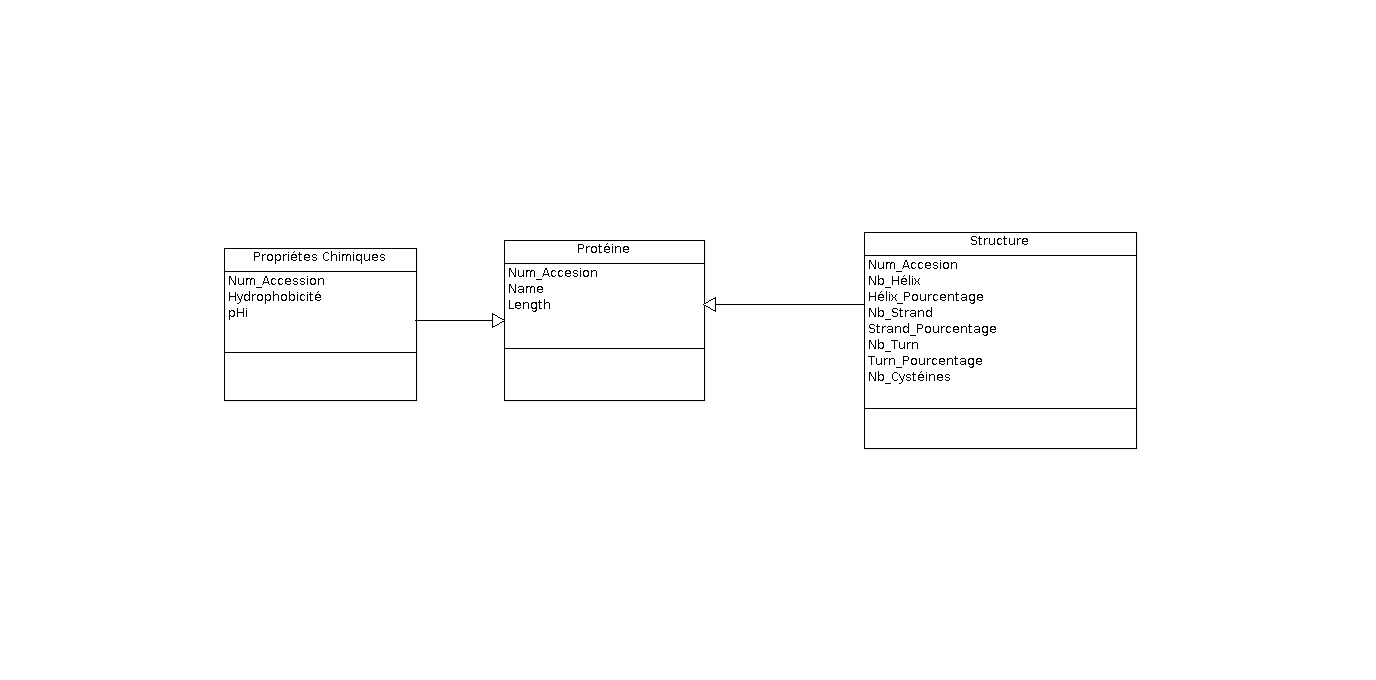
\includegraphics[width=20cm, height=10cm]{structure_etoile.png}\\[1cm]

\subsubsection*{Clusters}
\addcontentsline{toc}{subsection}{Clusters}
Nous avons choisi de réaliser un clustering hiérarchique car l'attribution de scores aux protéines nous paraissait particulièrement complexe, dans le cas de données non numérique, et fastidieux.\\
%de le cas du clustering par scores nous paraissait fastidieuse.\\

Enfin nous avons remarqué que certaines protéines n'étaient pas des protéines humaines mais appartenaient à des virus, nous les avons donc supprimées. De plus, certaines protéines n'avaient pas de structure secondaire, nous avons décidé de ne pas les prendre en compte pour la création de nos clusters.\\
\newline
Nous obtenons ainsi un fichier XML contenant uniquement les données que nous avons sélectionnées. Il contient environ 4000 protéines.\\

A partir de ce fichier et pour faciliter la création des clusters, nous avons décidé de créer trois tables.(cf figure table)
\begin{description}
\item[La table protéine] comprend toutes les données relatives à la protéine tel que le numéro d'accession, son nom complet, sa longueur et une liste contenant ses localisations.
\item[La table Structure] contient toutes les informations de structure de la protéine: le nombre et le pourcentage d'hélices, de feuillets et de coudes ainsi que le nombre de cystéines qu'elle possède.
\item[La table des propriétés chimiques] contient le pourcentage d'hydrophobicité et le pHi de la protéine.
\end{description}
Ses tables sont en fait des dictionnaires dans lesquels la clé est le numéro d'accession de la protéine. La valeur associée à la clé est un autre dictionnaire dans lequel les clés sont les noms des paramètres.

%
%\section*{Clusters}
%\addcontentsline{toc}{section}{Clusters}
%Nous avons choisi de réaliser un clustering hiérarchique car l'attribution de scores aux protéines nous paraissait particulièrement complexe dans le cas de données non numériques.\\%de le cas du clustering par scores nous paraissait fastidieuse.\\
%Ainsi, nous avons choisi 7 niveaux de clusterisation:
%\begin{enumerate}
%\item Taille de la chaîne (en nombre d'acides aminés)
%\item Structure tridimensionnelle (nombre d'hélices, de feuillets, de coudes et de cystéines)
%\item Pourcentage d'hydrophobicité
%\item pHi
%\item Localisation au niveau organe
%\end{enumerate}



%\subsubsection*{Taille de la chaîne}
%Les protéines sont constitués d'une succession d'acides aminés reliés entre eux par des liaisons peptidiques. La taille d'une protéine est ainsi définit par le nombre d'acides aminés qu'elle contient. Cette taille étant très variable, les protéines ayant des tailles très différentes n'auront pas les mêmes propriétés, ce critère constitue donc un bon premier niveau de clusterisation.
%
%Pour déterminer la distance entre deux protéines, nous calculons la distance de Manhattan et créons des clusters de façon arbitraires, tout en tentant de maintenir un nombre equivalent de proteines dans chacun des groupes créés. Nous obtenons ainsi X clusters de x proteines en moyennes.\\

%\subsubsection*{Localisation}
%Les protéines sont des constituants de notre organisme et participe à la composition de la matrice de chacun de nos organes, tissus ainsi que nos cellules. Elles peuvent avoir différentes fonctions spécifiques à leur localisation.\\

\subsection*{Taille de la chaîne}
\addcontentsline{toc}{subsection}{Taille de la cha\^ine}
Les protéines sont constituées d'une succession d'acides aminés reliés entre eux par des liaisons peptidiques. La taille d'une protéine est ainsi définie par le nombre d'acides aminés qu'elle contient. Cette taille étant très variable, les protéines ayant des tailles très différentes n'auront pas les m\^emes propriétés, ce critère constitue donc un bon premier niveau de clusterisation.

% et créons des clusters de façon arbitraires, tout en tentant de maintenir un nombre equivalent de proteines dans chacun des groupes créés. Nous obtenons ainsi X clusters de x proteines en moyennes
Pour que la formation des cluster se fasse rapidement, nous avons tout d'abord décidé de trier les protéines par longueur croissante. Puis nous avons regroupé ces dernières dans des cluster de 250 éléments.

\subsection*{Structure tridimensionnelle}
\addcontentsline{toc}{subsection}{Structure tridimensionnelle}
Une protéine peut être décrite par un enchaînement de structures secondaires (hélices alpha, feuillets beta et coude) qui ont une influence sur son repliement.\\
Les clusters de structure tridimensionnelle ont été créés à partir de chaque cluster de taille précédent.\\
Dans un premier temps, nous avons calculé la distance entre deux protéines gr\^ace à la distance de Manhattan.
Puis à partir de ces distances, nous avons établi une matrice que nous réduisons petit à petit en regroupant les protéines qui ont les distances les plus proches. Nous avons répété l'opération jusqu'à diviser chaque cluster de taille en quatre groupes de cluster de structure tridimensionnelle.

\subsection*{Hydrophobicité}
\addcontentsline{toc}{subsection}{Hydrophobicité}
L'hydrophobicité d'une protéine est déterminée à partir du nombre d'acides aminés hydrophobes qu'elle possède.
Nous avons calculé un index d'hydrophobicité (GRAVY: Grand average of hydropathicity index,Kyte and Doolittle) qui indique la solubilité d'une protéine. Si la valeur est positive, la protéine est hydrophobe, sinon elle est hydrophile.
Son caractère hydrophobe ou hydrophile influence :
\begin{itemize}
\item Sa localisation au niveau cellulaire (cytoplasme ou membrane)
\item Son repliement (acides aminés hydrophobes à l'intérieur ou l'extérieur de la protéine selon sa localisation cellulaire) 
\end{itemize}
La formation des clusters d'hydrophobicité suit le m\^eme procédé que celui de la structure tridimensionnelle. Nous arr\^etons la formation lorsque chaque cluster de structure tridimensionnelle a été divisé en quatre.

\subsection*{Nombre de cystéines}
\addcontentsline{toc}{subsection}{Nombre de cystéines}
Les ponts disulfures se forment au sein d'une protéine entre deux cystéines et créent des liaisons inter-chaines. Ils ont donc une influence sur la structure tridimensionnelle de la protéine.\\
La formation des clusters de cystéine suit le m\^eme procédé que celui de la structure tridimensionnelle. Nous arr\^etons la formation lorsque chaque cluster d'hydrophobcité a été divisé en quatre.

\subsection*{pHi}
\addcontentsline{toc}{subsection}{pHi}
Le pHi est le pH isoéléctrique d'une protéine, c'est à dire le pH auquel cette protéine a une charge nulle et donc limite son déplacement dans un champ électrique physiologique.
Au dessus de ce pH, la protéine est chargée négativement (pH basique) et inversement, en dessous elle est chargée positivement (pH acide).\\
Les peptides composant la protéines sont des molécules chargées, à cause de leur groupement C (carbone) et N (azote) terminaux et les groupements fonctionnels des carbones alpha des acides aminés polaire. L'association de ses peptides détermines le pHi de la protéines car c'est le point de pH où les charges positives et négatives de l'ensemble de la protéines est nulle, soit que les charge positive et négative se compensent.\\
Ainsi lorsqu'une protéine est dans un milieu égale à son pHi cela met en évidence différentes propriétés, telles que:
\begin{itemize}
\item Sa solubilité qui est minimale,
\item Sa mobilité électrophorétique qui lui permet de migrer plus vers un milieu qu'un autre,
\item Son isoélectrofocalisation (IEF) qui repose sur ses peptides amphotères qui vont charger la protéines négativement ou positivement selon le milieu.
\end{itemize}
La formation des clusters de pHi suit le m\^eme procédé que celui des précédentes formations. Nous arr\^etons la formation lorsque chaque cluster de cystéines a été divisé en quatre.

\subsection*{Localisation}
\addcontentsline{toc}{subsection}{Localisation}
Les protéines sont des constituants de nos organes et participent à la composition de la matrice de chacun de nos organes, tissus ainsi que nos cellules.\\% Elles peuvent avoir différentes fonctions:
%\begin{itemize}
%\item messagers universels (entre deux organes),
%\item bâtisseurs omnipotents (Enzyme, Co-Enzyme),
%\item armes de défense active (Anticorps, Cytokines),
%\item base de la contraction musculaire (Actine, Myosine),  
%\item pompe "aspirantes-souflantes" (dans le sang: dispersent les aggloméra de lipide et pompent l'eau qui s'échappe des vaisseaux). \\
%\end{itemize}
Nous avons fait le choix de nous restreindre au niveau organique. Un protéines à des fonctions déterminées qui peuvent être utile dans différents organes, voisin ou non. 
\\

%\subsubsection*{Conformation}
%Une protéine peut être décrite par un enchaînement de structures secondaires régulières et répétées (hélices alpha, feuillets bêta et coude bêta) qui influence la stabilité de son reploiement global.\\
%Les hélices alpha et les feuillets bêta sont formés par une configuration régulière de liaisons hydrogènes entre les groupements peptidiques \ce{N-H} et \ce{C=O} des résidus d'aminoacides. Leur formation est Ces liaisons sont impliquées dans de nombreux résidus consécutifs.
%\\

%\subsubsection*{Nombre de cystéine}
%Les ponts disulfures se forment au sein d'une protéine entre deux cystéines (lien \ce{S-S}) et créent des liaisons inter ou intra-chaines post-traductionnelle. Ce sont des liaisons covalentes formées par l'oxydation des groupements thiols (\ce{-SH}) qui donne une molécule de cystine.\\
%Cette architecture est un élément de la structure tertiaire ou quaternaire de la protéine en présence de dioxygène (\ce{O2-O2}).Elle permet de stabiliser la protéine en liant les chaînes pepidiques ou sous-unités de la protéines ou en  son repliement spécifique (site actif enzymatique). Elle permet ainsi de réduire son entropie configurationnelle.
%\\

%\subsubsection*{Hydrophobicité}
%L'hydrophobicité d'une protéine est déterminée à partir du nombre d'acides aminés hydrophobes qu'elle possède.
%Nous avons calculé un index d'hydrophobicité (GRAVY: Grand average of hydropathicity index,Kyte and Doolittle) qui indique la solubilité d'une protéine. Si la valeur est positive, la protéine est hydrophobe, sinon elle est hydrophile.
%Son caractère hydrophobe ou hydrophile influence :
%\begin{itemize}
%\item sa localisation au niveau cellulaire (cytoplasme ou membrane)
%\item son repliement (acides aminés hydrophobes à l'intérieur ou l'extérieur de la protéine selon sa localisation cellulaire) \\
%\end{itemize}

%\subsubsection*{pHi}
%Le pHi est le pH isoéléctrique d'une protéine, c'est à dire le pH auquel cette protéine a une charge nulle et donc limite son déplacement dans un champ électrique physiologique.
%Au dessus de ce pH, la protéine est chargée négativement (pH basique) et inversement, en dessous elle est chargée positivement (pH acide).\\
%Les peptides composant la protéines sont des molécules chargées, à cause de leur groupement \ce{C} (carbone) et \ce{N} (azote) terminaux et les groupements fonctionnels des carbones alpha des acides aminés polaire. L'association de ses peptides détermines le pHi de la protéines car c'est le point de pH où les charges positives et négatives de l'ensemble de la protéines est nulle, soit que les charge positive et négative se compensent.\\
%Ainsi lorsqu'une protéine est dans un milieu égale à son pHi cela met en évidence différentes propriétés, tels que:
%\begin{itemize}
%\item sa solubilité qui est minimale,
%\item sa mobilité électrophorétique qui lui permet de migrer plus vers un milieu qu'un autre,
%\item son isoélectrofocalisation (IEF) qui repose sur ses peptides amphotères qui vont charger la protéines négativement ou positivement selon le milieu.\\
%\end{itemize}
%
%Une protéine a des fonctions déterminées qui peuvent être utiles dans différents organes, voisins ou non. \\
%Le principal problème qui s'est posé pour la formation des clusters de localisation était d\^u au fait qu'une protéine peut avoir plusieurs localisations.
%Pour former les clusters de localisation, nous avons donc déterminé les similarités entre les différentes localisations des protéines. Plus elles avaient de localisations communes, plus elles étaient similaires.\\
%A partir de là nous avons pu créer les clusters à partir de chaque cluster de pHi.





